\documentclass[a4paper,12pt]{report}
\usepackage[T2A]{fontenc}
\usepackage[utf8]{inputenc}
\usepackage[english,russian]{babel}
\usepackage{graphicx}
\usepackage{wrapfig}
\usepackage{mathtext} 				% русские буквы в фомулах
\usepackage{amsmath,amsfonts,amssymb,amsthm,mathtools} % AMS
\usepackage{icomma} % "Умная" запятая: $0,2$ --- число, $0, 2$ --- перечисление
\usepackage{capt-of}
\usepackage{appendix}
\usepackage{multirow}
\usepackage{hyperref}
\usepackage{floatrow}
\usepackage[left=2cm,right=2cm,
    top=2cm,bottom=2cm,bindingoffset=0cm]{geometry}
\usepackage{multicol} % Несколько колонок
\usepackage{gensymb}
\title{Отчёт по лабораторной работе № 5.4.1. 

Определение энергии $\alpha$-частиц по величине их пробега в воздухе.}
\author{Плюскова Н.А. Б04-004 }
\date{\today}
\begin{document}
\maketitle
\section*{1. Аннотация}



\section*{2. Теоретические сведения}
	При $\alpha$-распаде исходное родительское ядро испускает ядро гелия и превращается в дочернее ядро, число протонов и число протонов уменьшается на две единицы. Функциональная свзяь между энергией $\alpha$-частицы $E$ и периодом полураспада радиоактивного ядра $T_{1/2}$ хорошо описывается формулой
	\begin{equation*}
		 \lg T_{1/2} = \frac{a}{\sqrt{E}} + b.
	\end{equation*}
	Экспоненциальный характер этого процесса возникает вследствие экспоненциального затухания волновой функции в области под барьером, где потенциальная энергия больше энергии частицы.
	
	Для описания связи между энергией $\alpha$-частицы и ее пробегом пользуются эмпирическими соотношениями. В диапазоне энергий $\alpha$-частиц от 4 до 9 МэВ эта связь хорошо описывается выражением:
	\begin{equation*}
		\label{eq:R(E)}
		R = 0,32E^{3/2}
	\end{equation*}
\section*{3. Экспериментальная установка}
В данной работе пробег $\alpha$-частиц в воздухе определяется тремя способами: помощью счетчика Гейгера (рис.1а), сцинтилляционного счетчика (рис.1б) и ионизационной камеры (рис.1в).
	
        \begin{figure*}[h!]
            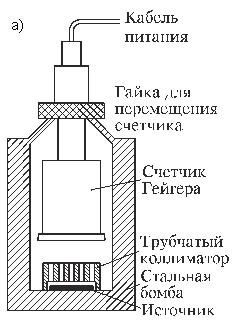
\includegraphics[width=.3\textwidth]{ustanovka1.pdf}\hfill
            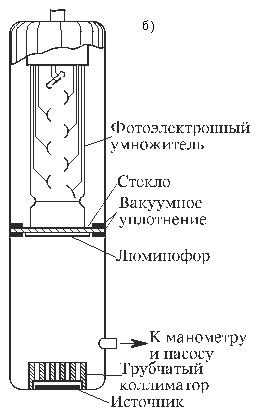
\includegraphics[width=.3\textwidth]{ustanovka2.pdf}\hfill
            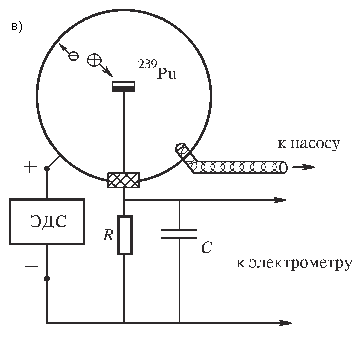
\includegraphics[width=.3\textwidth]{ustanovka3.pdf}
            \caption{Экспериментальные установки}
        \end{figure*}
        
	В качестве источника $\alpha$-частиц используется ${239}$Pu с периодом полураспада $T_{1/2} = 2,44 \cdot 10^4$ лет. Альфа-частицы, испускаемые ${239}$Pu состоят их трех моноэнергетических групп, различие между которыми лежит в пределах 50 кэВ. При той точности, которая достигается в наших опытах, их можно считать совпадающими по энергии, равной 5,15 МэВ.
	
	
\section*{4. Ход работы}
\subsection*{4.1 Исследование пробега $\alpha$-частиц с помощью счетчика Гейгера}

Измерим зависимость скорости счета $N$ от расстояния $x$ между источником и счетчиком:

\begin{table}[H]
\begin{tabular}{|c|c|c|}
\hline
$t$, с & $x$ ,мм & $N$, имп \\ \hline
54   & 10    & 781    \\ \hline
50   & 10,5  & 793    \\ \hline
45   & 11    & 743    \\ \hline
51   & 11,5  & 791    \\ \hline
51   & 12    & 737    \\ \hline
52   & 12,5  & 797    \\ \hline
48   & 13    & 696    \\ \hline
47   & 13,5  & 710    \\ \hline
58   & 14    & 853    \\ \hline
52   & 14,5  & 783    \\ \hline
51   & 15    & 737    \\ \hline
53   & 15,5  & 734    \\ \hline
59   & 16    & 788    \\ \hline
57   & 16,5  & 789    \\ \hline
67   & 17    & 813    \\ \hline
68   & 17,5  & 660    \\ \hline
95   & 18    & 662    \\ \hline
102  & 18,5  & 326    \\ \hline
122  & 19    & 100    \\ \hline
104  & 19,5  & 35     \\ \hline
101  & 22    & 26     \\ \hline
\end{tabular}
\end{table}

Построим график зависимости $N = N(x)$:

	\begin{figure}[H]
		\centering
		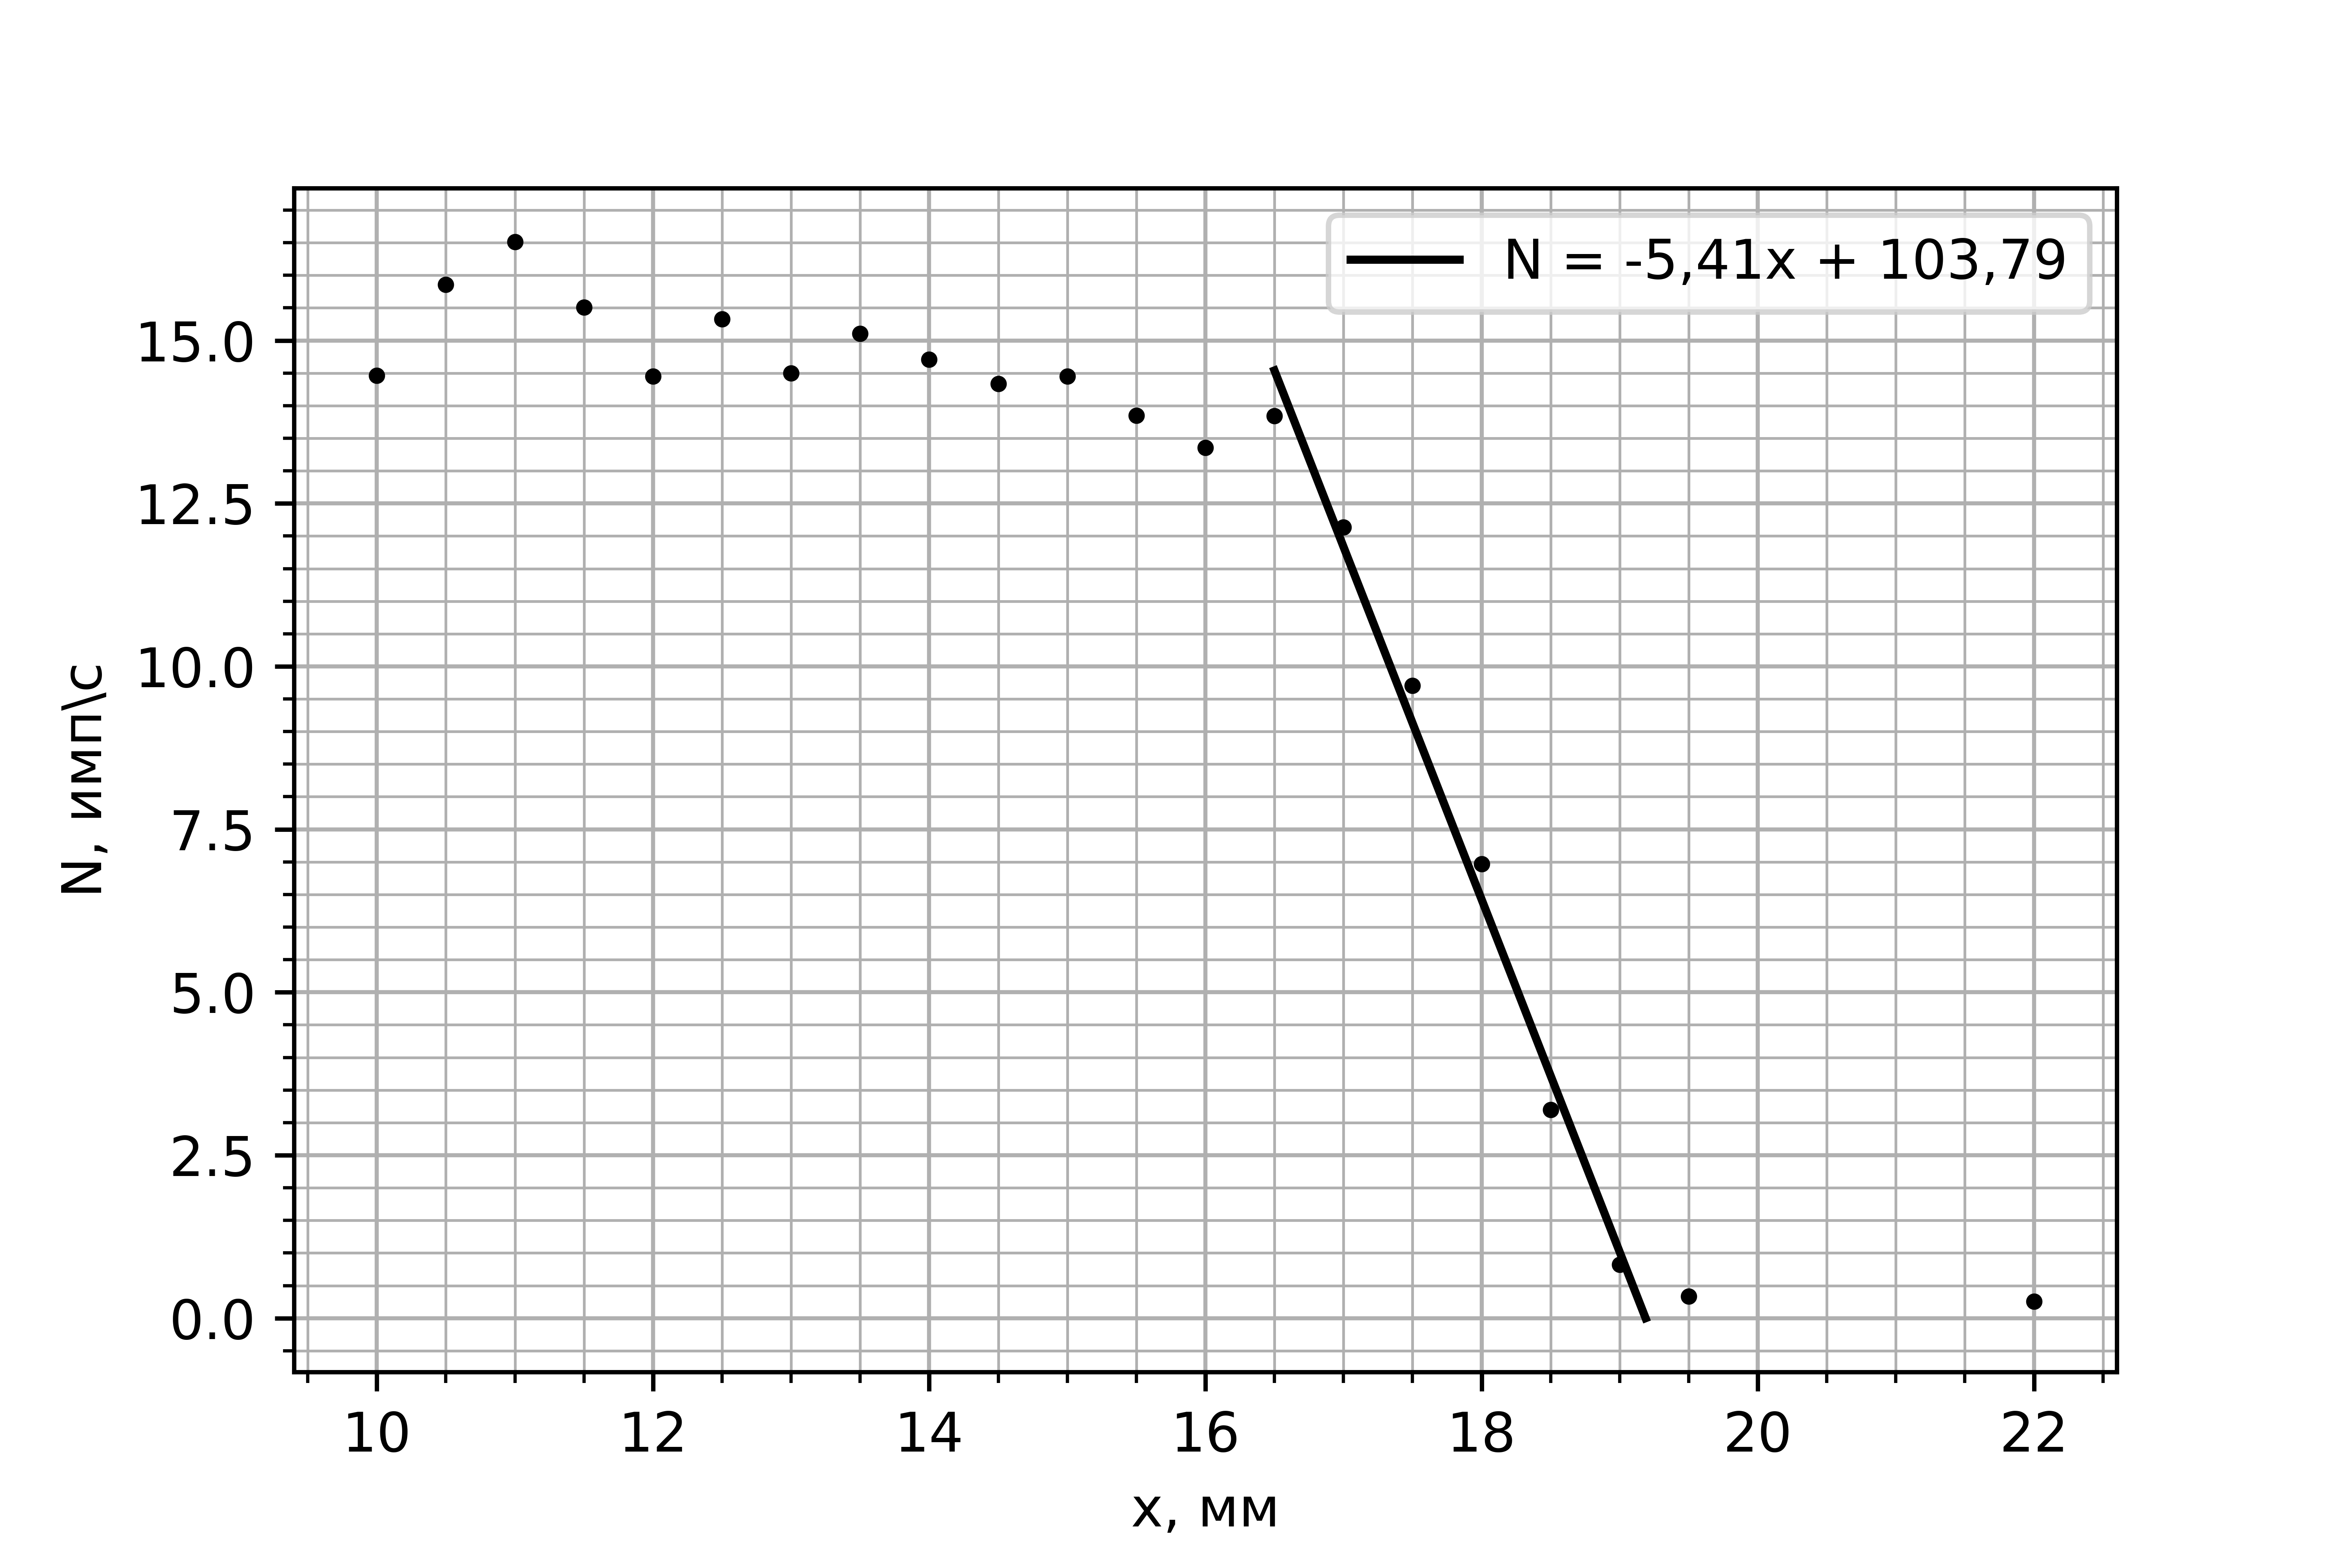
\includegraphics[width=0.7\linewidth]{N(x).png}
		\caption{Зависимость $N = N(x)$}
	\end{figure}

Наклонную часть графика аппроксимируем линейной функцией и экстраполируем полученую прямую до пересечения с осью абсцисс. Отсюда получаем экстраполированную длину пробега с погрешностью, определяемую из МНК:

\begin{center}
    $R_{e} \approx (19,2 \pm 0,9)$ мм $\rightarrow R'_{e} = \rho R_{e} = (2,41 \pm 0,11)$ мг/см$^2$
\end{center}
	
Среднюю длину пробега оценим как координату середины прямой по оси абсцисс:

$R_{av}\approx (17,8\pm0,9)$ мм $ \rightarrow R'_{av}=\rho R_{av}=(2,17\pm0,10)$ мг/см$^2$. 

Отметим, что истинный пробег $\alpha$-частиц больше измеренного, так как часть энергии частиц тратится на прохождение слюдяной пластинки, прикрывающей счетчик, и пленки, закрывающей источник.

\subsection*{4.2 Определение пробега $\alpha$-частиц с помощью сцинтилляционного счетчика}

Измерим зависимость скорости счета $N$ от давления $P$ в камере:

\begin{table}[H]
\begin{tabular}{|c|c|c|c|c|}
\hline
$t$, с & $P$ ,торр & $\sigma_{P}$ ,торр          & $N$    & $\sigma_N$ \\ \hline
10   & 328,6   & \multirow{10}{*}{2,5} & 4    & 2      \\ \cline{1-2} \cline{4-5} 
10   & 278,6   &                       & 70   & 8      \\ \cline{1-2} \cline{4-5} 
10   & 248,6   &                       & 325  & 18     \\ \cline{1-2} \cline{4-5} 
10   & 228,6   &                       & 728  & 27     \\ \cline{1-2} \cline{4-5} 
10   & 198,6   &                       & 1291 & 36     \\ \cline{1-2} \cline{4-5} 
10   & 178,6   &                       & 1690 & 41     \\ \cline{1-2} \cline{4-5} 
10   & 168,6   &                       & 1921 & 44     \\ \cline{1-2} \cline{4-5} 
10   & 148,6   &                       & 2199 & 47     \\ \cline{1-2} \cline{4-5} 
10   & 129,6   &                       & 2624 & 51     \\ \cline{1-2} \cline{4-5} 
10   & 118,6   &                       & 2714 & 52     \\ \hline
\end{tabular}
\end{table}

Построим график зависимости $N = N(P)$:

	\begin{figure}[H]
		\centering
		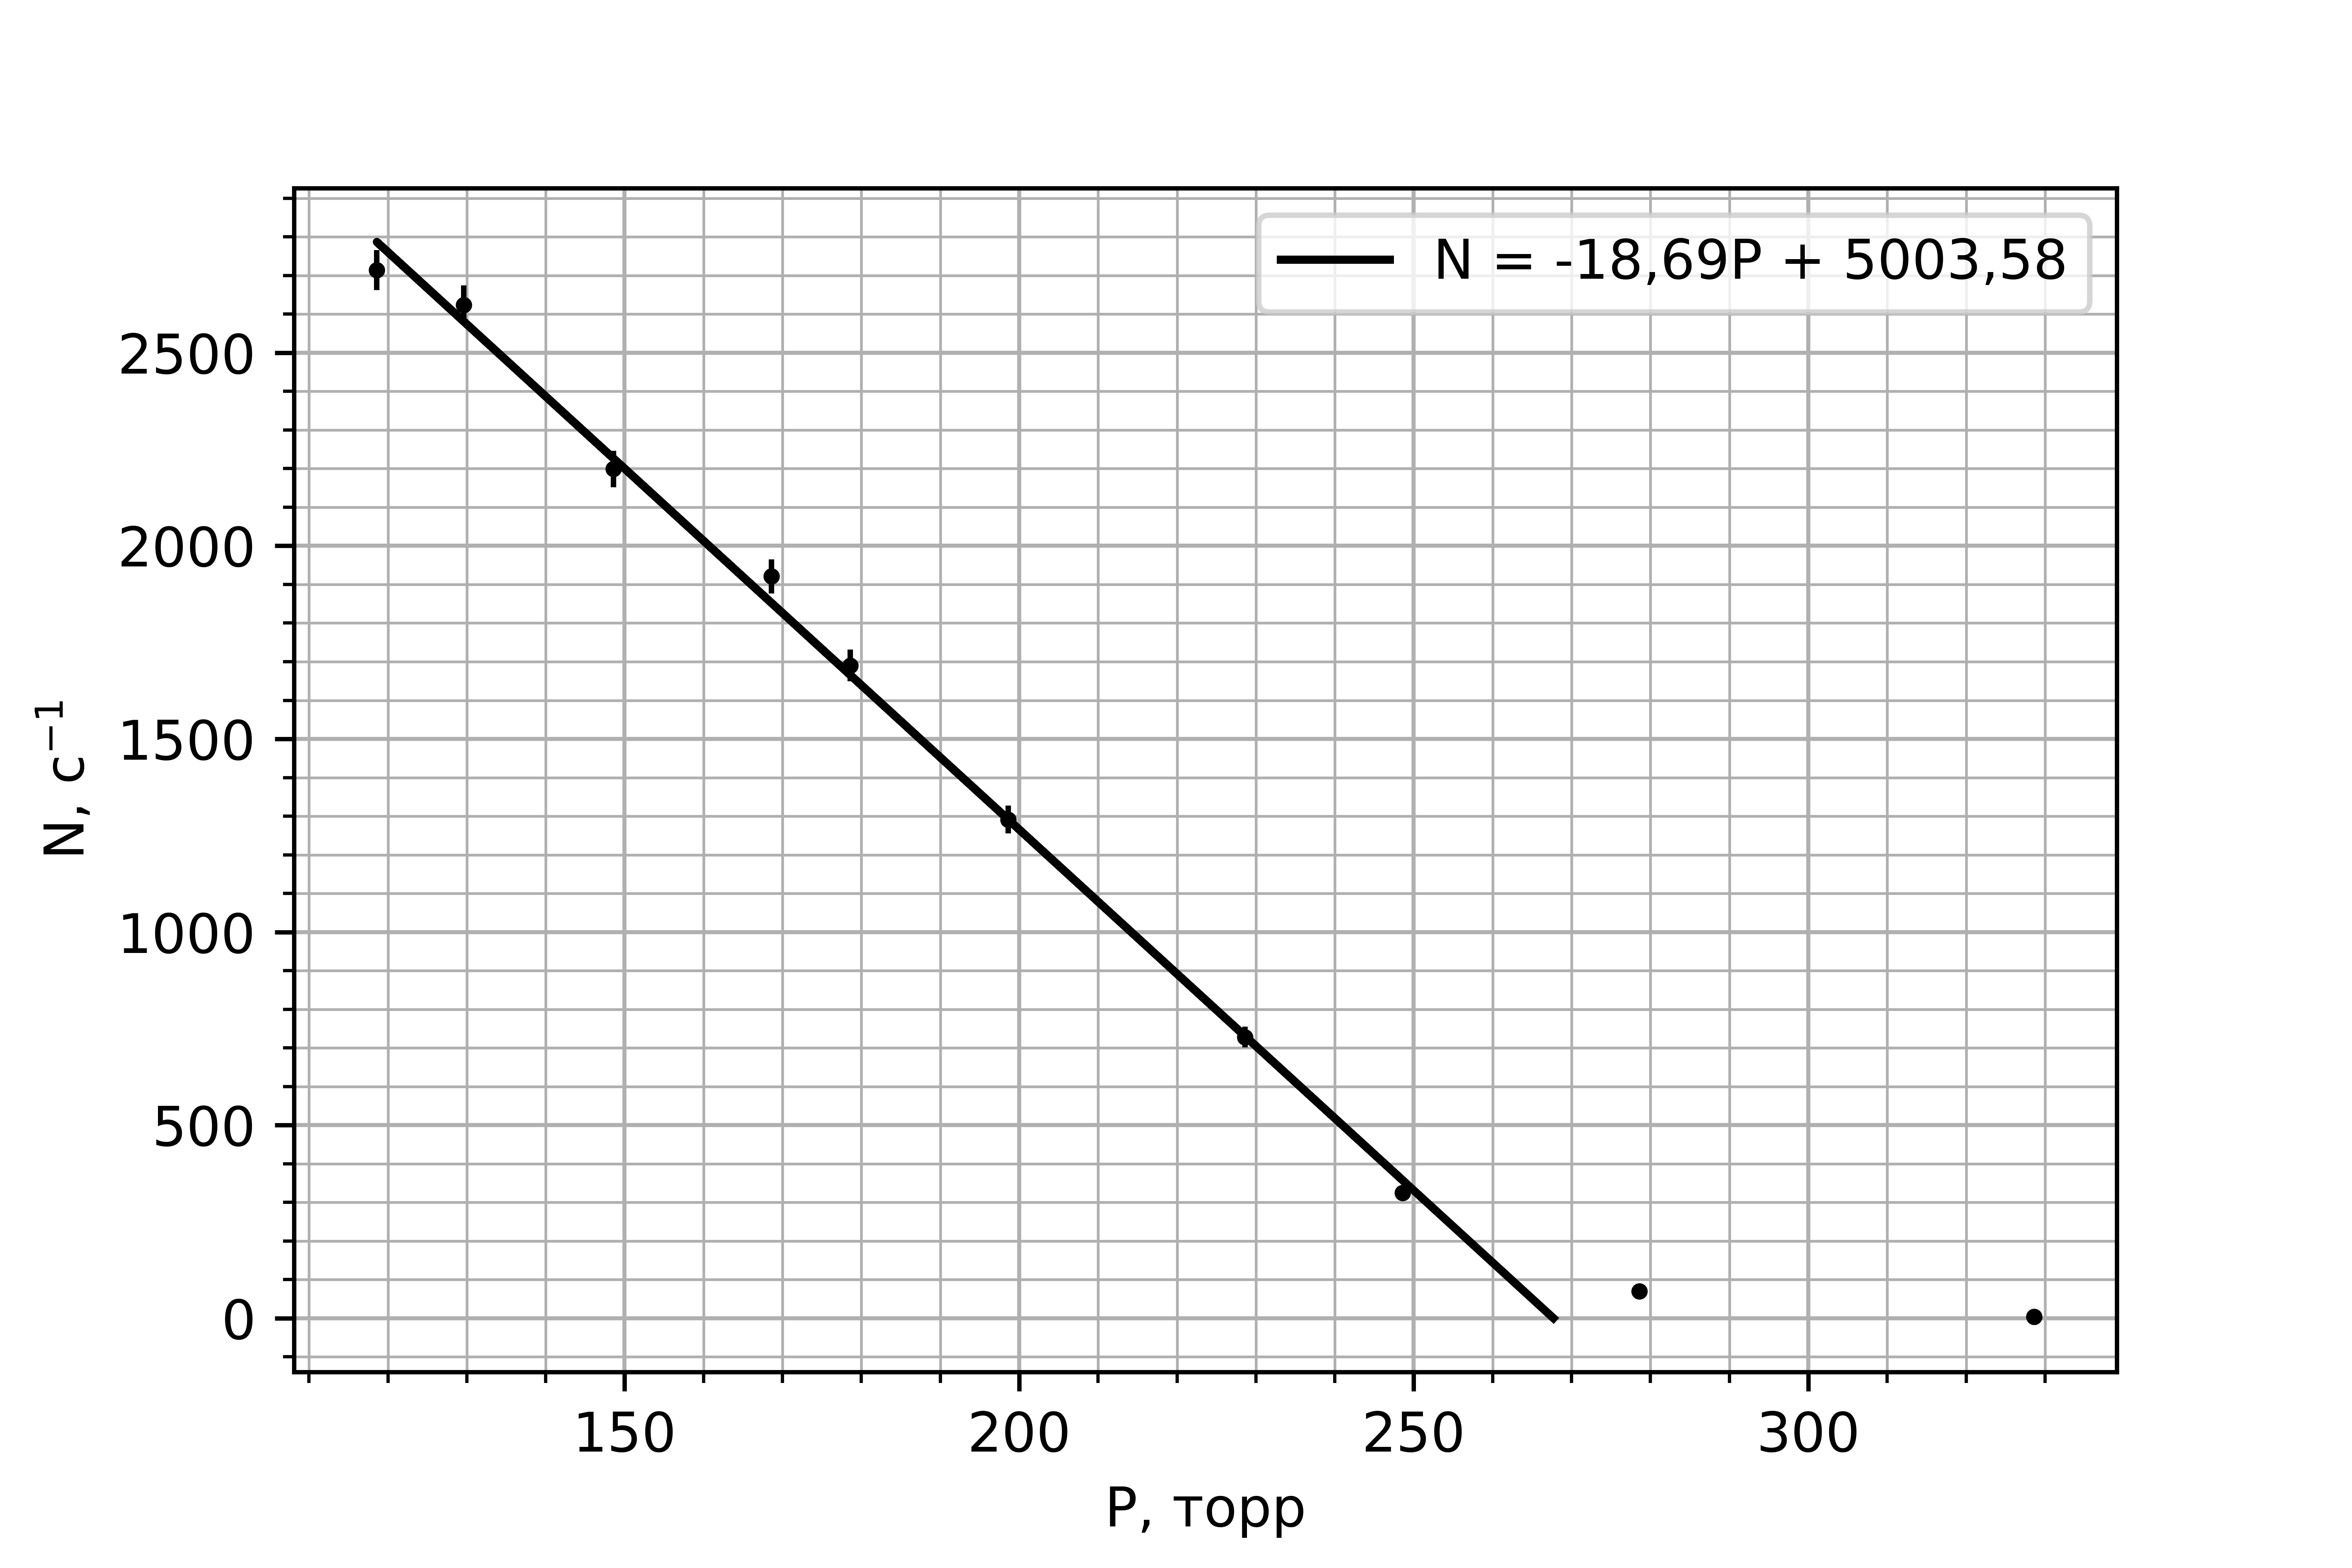
\includegraphics[width=0.7\linewidth]{N(P).png}
		\caption{Зависимость $N = N(P)$}
	\end{figure}

Из графика получим: $P_{\text{0}}\approx(267,7\pm 2,3)$ торр

Экстраполированная длина пробега находится по формуле:
\begin{center}
    $R_{э} = R_{l} \cfrac{\rho}{\rho_0} =R_{l} \cfrac{PT_0}{P_0T} \approx 3,51 \pm 0,52$ cм $\rightarrow R'_{э} \approx 4,3 \pm 0,64$ мг/см$^2$,
\end{center}

где $R_l = 90$ мм - пробег при н.у.

Погрешность $R$ считалась по формуле:
\begin{equation*}
    \sigma_{R} = \sqrt{(R_{l}\cdot\frac{T}{PT_{0}}\cdot\sigma_{P_{0}})^2 + (R_{l}\cdot\frac{P_{0}T}{PT_{0}^2}\cdot\sigma_{T_{0}})^2}
\end{equation*}

Оценим энергию $\alpha$-частицы по эмпирической формуле: 
	\begin{equation*}
		R = 0,32E^{3/2}
	\end{equation*}
	
Откуда получаем:
\begin{center}
    $ E \approx(4,94\pm0,49) $ МэВ
\end{center}

Погрешность энергии считалась по формуле:
\begin{equation*}
    \sigma_{E} = \frac{2\cdot \sigma_{R}}{3\cdot0,32\cdot R^{\frac{1}{3}}}
\end{equation*}

\subsection*{4.3 Определение пробега $\alpha$-частиц с помощью ионизационной камеры}

Измерим зависимость величины тока $I$ от давления $P$ в камере:

\begin{table}[H]
\begin{tabular}{|c|c|c|c|}
\hline
$P$ ,торр & $\sigma_P$ ,торр          & $I$, А & $\sigma_I$, А \\ \hline
728,6   & \multirow{17}{*}{2,5} & 880  & 5         \\ \cline{1-1} \cline{3-4} 
698,6   &                       & 883  & 5         \\ \cline{1-1} \cline{3-4} 
678,6   &                       & 887  & 5         \\ \cline{1-1} \cline{3-4} 
678,6   &                       & 887  & 5         \\ \cline{1-1} \cline{3-4} 
658,6   &                       & 898  & 5         \\ \cline{1-1} \cline{3-4} 
638,6   &                       & 900  & 5         \\ \cline{1-1} \cline{3-4} 
628,6   &                       & 901  & 5         \\ \cline{1-1} \cline{3-4} 
618,6   &                       & 904  & 5         \\ \cline{1-1} \cline{3-4} 
598,6   &                       & 904  & 5         \\ \cline{1-1} \cline{3-4} 
578,6   &                       & 907  & 5         \\ \cline{1-1} \cline{3-4} 
578,6   &                       & 907  & 5         \\ \cline{1-1} \cline{3-4} 
558,6   &                       & 905  & 5         \\ \cline{1-1} \cline{3-4} 
538,6   &                       & 890  & 5         \\ \cline{1-1} \cline{3-4} 
528,6   &                       & 883  & 5         \\ \cline{1-1} \cline{3-4} 
518,6   &                       & 870  & 5         \\ \cline{1-1} \cline{3-4} 
498,6   &                       & 836  & 5         \\ \cline{1-1} \cline{3-4} 
478,6   &                       & 800  & 2         \\ \hline
\end{tabular}
\hspace{1cm}
\begin{tabular}{|c|c|c|c|}
\hline
$P$ ,торр & $\sigma_P$ ,торр          & $I$, А & $\sigma_I$, А  \\ \hline
428,6   & \multirow{17}{*}{2,5} & 698  & 2         \\ \cline{1-1} \cline{3-4} 
378,6   &                       & 605  & 2         \\ \cline{1-1} \cline{3-4} 
328,6   &                       & 507  & 2         \\ \cline{1-1} \cline{3-4} 
298,6   &                       & 449  & 1         \\ \cline{1-1} \cline{3-4} 
278,6   &                       & 416  & 1         \\ \cline{1-1} \cline{3-4} 
248,6   &                       & 362  & 1         \\ \cline{1-1} \cline{3-4} 
228,6   &                       & 332  & 1         \\ \cline{1-1} \cline{3-4} 
198,6   &                       & 282  & 1         \\ \cline{1-1} \cline{3-4} 
178,6   &                       & 252  & 1         \\ \cline{1-1} \cline{3-4} 
129,6   &                       & 172  & 0         \\ \cline{1-1} \cline{3-4} 
118,6   &                       & 155  & 1         \\ \cline{1-1} \cline{3-4} 
98,6    &                       & 124  & 1         \\ \cline{1-1} \cline{3-4} 
79,6    &                       & 97   & 0         \\ \cline{1-1} \cline{3-4} 
78,6    &                       & 94   & 0         \\ \cline{1-1} \cline{3-4} 
58,6    &                       & 67   & 0         \\ \cline{1-1} \cline{3-4} 
38,6    &                       & 37   & 0         \\ \cline{1-1} \cline{3-4} 
26,6    &                       & 19   & 0         \\ \hline
\end{tabular}
\end{table}

Построим график зависимости $I = I(P)$:

	\begin{figure}[H]
		\centering
		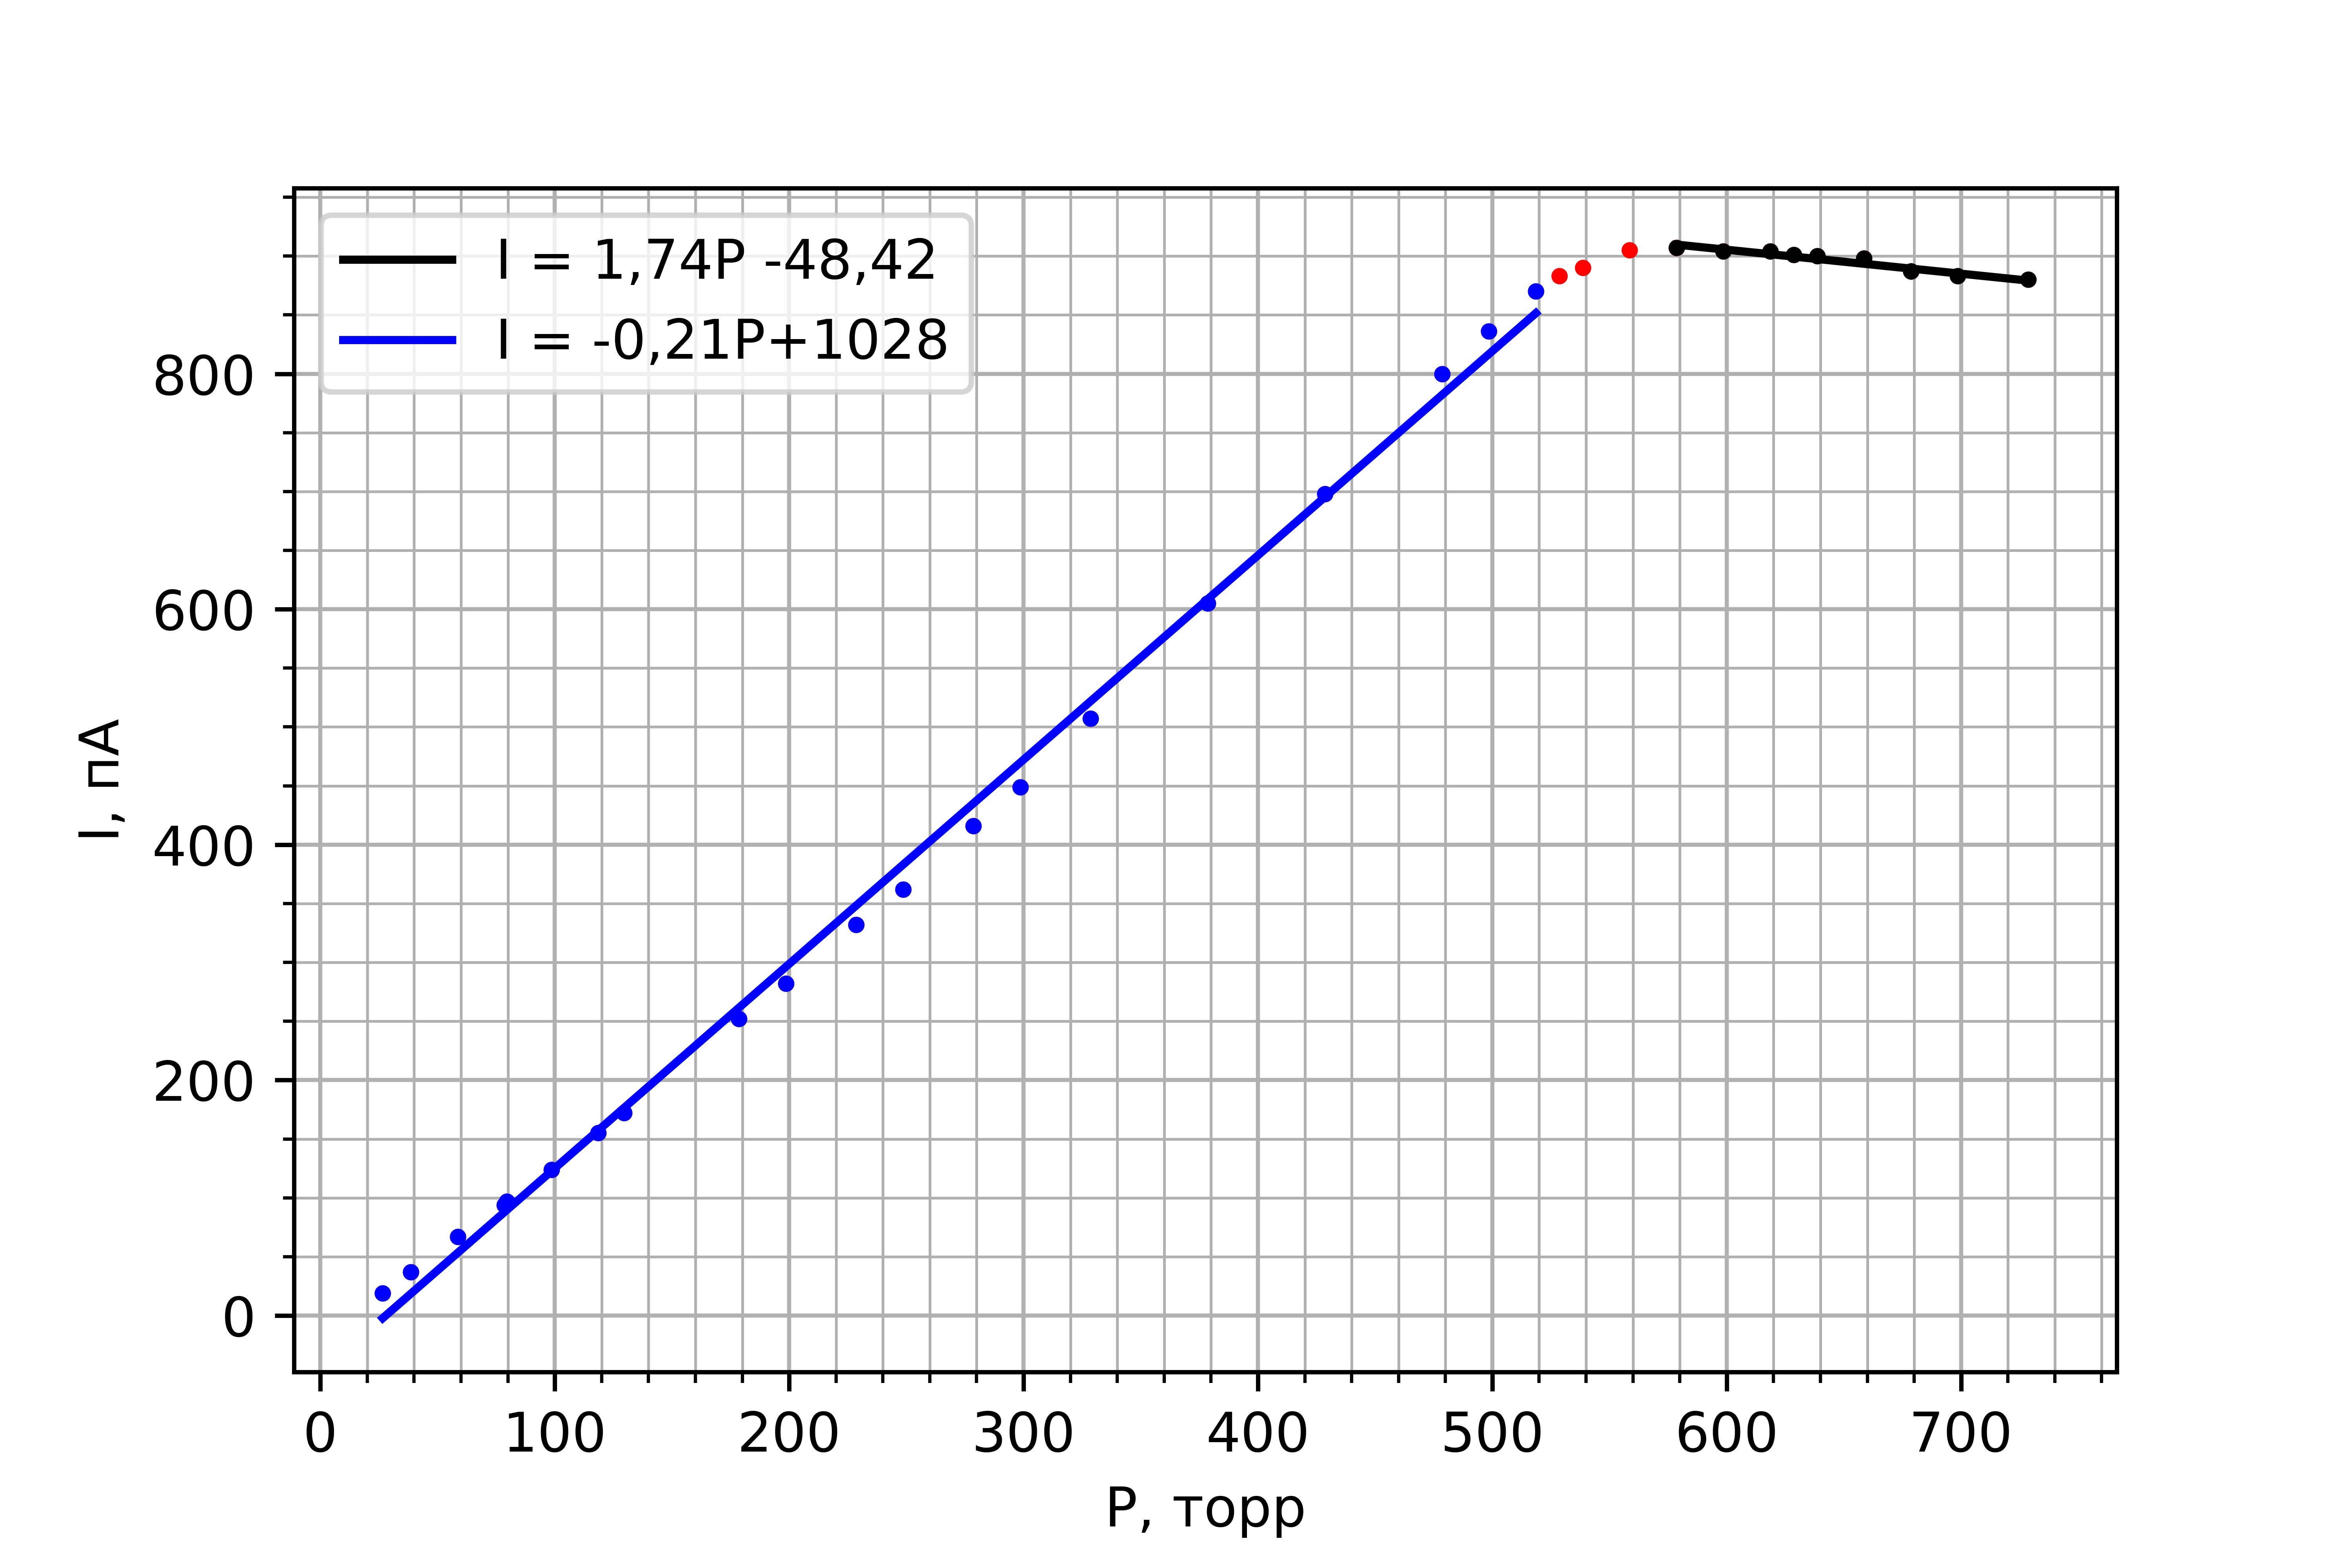
\includegraphics[width=0.7\linewidth]{I(P).png}
		\caption{Зависимость $I = I(P)$}
	\end{figure}

По графику определим давление $P_{0}$, при котором $\alpha$ - частицы заканчивают свой пробег внутри газа. Для этого построим две прямых, соответствующих линейным участкам графика. Их пересечение дает нам значение 
	
\begin{center}
    $P_{0} = \cfrac{b_2 - b_1}{a_1 - a_2} \approx (562.2\pm 5.1)\text{ торр}$
    
\end{center}
     
Так как пробег $ R_l = 5 $ см задается размером камеры, приведем его к н.у.:

\begin{center}
    $R_{э} = R_{l} \cfrac{\rho}{\rho_0} = R_l \cfrac{PT_0}{P_0T} \approx (3,84 \pm 0,50)$ cм $\rightarrow R'_{э} \approx (4,71 \pm 0,61)$ мг/см$^2$
\end{center}

Погрешность $R$ считалась по формуле:
\begin{equation*}
    \sigma_{R} = \sqrt{(R_{l}\cdot\frac{T}{PT_{0}}\cdot\sigma_{P_{0}})^2 + (R_{l}\cdot\frac{P_{0}T}{PT_{0}^2}\cdot\sigma_{T_{0}})^2}
\end{equation*}

Оценим энергию $\alpha$-частицы по эмпирической формуле: 
	\begin{equation*}
		R = 0,32E^{3/2}
	\end{equation*}
	
Откуда получаем:
\begin{center}
    $ E \approx (5,24 \pm 0,45) $ МэВ
\end{center}


Погрешность энергии считалась по формуле:
\begin{equation*}
    \sigma_{E} = \frac{2\cdot \sigma_{R}}{3\cdot0,32\cdot R^{\frac{1}{3}}}
\end{equation*}
\section*{5. Выводы}
В работе был измерен пробег альфа-частиц от $ ^{239}  $Pu тремя способами: с помощью торцевого счетчика Гейгера, сцинтилляционного счетчика и ионизационной камеры. По полученным данным была определена энергия альфа - частиц.

При работе с ионизационной камерой и сцинтилляционным счетчиком пробег и энергия получились близкими к ожидаемым в пределах погрешности (из таблиц при $ E = 5 $ МэВ получаем $ R = 3,29 $ см для воздуха). При работе со счетчиком Гейгера значение пробега ниже табличных. Это можно объяснить тем, что часть энергии альфа-частиц тратится на прохождение слюдяной пластинки, прикрывающей счетчик, и пленки, закрывающей источник. Толщину пленки можно оценить из соотношения $R'_{сцинт} = R'_{гейг} + 0,2R_{пленк} \rightarrow R_{пленк} \approx 9,45$ мг/см$^2$.

\end{document}
